%% ------------------------------------------------------------------------- %%
\chapter{Fundamentação Teórica}
\label{cap:fundamentacao-teorica}

O problema de remoção de ruído telúrico em sinais astronômicos é de natureza interdisciplinar, o que implica na necessidade de compreender tanto aspectos da teoria astronômica de espectros estelares, quanto aspectos relativos às representações e manipulações computacionais relacionadas ao problema.
Neste capítulo são descritos conceitos básicos em espectroscopia astronômica, principalmente estelar, e algoritmos de processamento de sinais digitais utilizados na pesquisa, que em conjunto caracterizam o problema da contaminação telúrica de espectros estelares e sua possível solução através de técnicas de filtragem.

\section{Espectroscopia Astronômica} \label{astronomic-spectroscopy}

% estrelas e radiação eletromagnética
Estrelas são corpos celestes que consistem de esferas de gás ionizado que são mantidas íntegras pela sua gravidade. Uma fonte fundamental de energia das estrelas é através de reações nucleares, principalmente a fusão de hidrogênio em hélio. A energia resultante desta fusão nuclear é emitida para o espaço em grande parte como radiação eletromagnética \citep{estrelas-ufrgs}.   

% propagação da radiação e chegada na atmosfera/terra
A radiação da estrela se propaga pelo meio interestelar como um fluxo de partículas denominadas fótons. Quando no espaço, estes fótons atingem o limite de velocidade universal, a velocidade da luz $\textit{c} \approx 3 \times 10^8$ m/s. Os fótons se aproximam da Terra nesta velocidade, mas assim que entram em contato com a atmosfera terrestre começam a interagir com moléculas como o oxigênio e o vapor de água \citep{wiki:photon}. Estas moléculas de gás podem absorver os fótons do sinal estelar, e consequentemente, alterar a quantidade de informação emitida por uma estrela que alcança a superfície terrestre \citep{wiki:telluric-contamination}.

% como a radiação é observada (primeira menção de instrumentos)
Os fótons que alcançam a superfície terrestre são medidos instrumentalmente, e essa captura de sinal é fundamental para estudos em astronomia observacional. Um dos instrumentos utilizados para fazer observações a partir do solo são os espectrógrafos, presentes em muitos telescópios. 

% como o espectrógrafo gera um espectro e utilização na astronomia (amarra os novos parágrafos com o texto antigo)
Este instrumento tem a capacidade de dividir a radiação eletromagnética de um objeto celeste em seus respectivos comprimentos de onda, resultando em um espectro: um mapa de radiação em função do comprimento de onda. Na astronomia, diversos corpos celestes podem ser o objeto de estudo de observações espectrais, como estrelas, planetas, nebulosas, galáxias e núcleos galácticos ativos.  

% A espectroscopia é a técnica de dividir a luz, ou mais precisamente, a radiação eletromagnética, proveniente de um objeto, em seus comprimentos de onda constituintes, o que resulta na formação de um mapa de radiação em função do comprimento de onda denominado espectro. Quando aplicada na astronomia, a espectroscopia tem como objeto de estudo o espectro de radiação eletromagnética de diversos corpos celestes, como estrelas, planetas, nebulosas, galáxias e núcleos galácticos ativos.

% tipos de espectro
Essa variedade de objetos celestes produz diferentes espectros, que podem ser divididos em três tipos principais: contínuo, de absorção e de emissão. Um espectro contínuo é uma função que tem como domínio todos os comprimentos de ondas do espectro eletromagnético.
Ele é gerado pela observação de um corpo opaco quente, que seria o equivalente a observar diretamente o núcleo de uma estrela sem intervenção de matéria entre estrela e observador. Um espectro de absorção, ou espectro de linhas escuras, é gerado por um gás transparente em frente ao corpo opaco quente e mais frio que este, e está associado à absorção dos fótons da radiação estelar em determinados comprimentos de onda. E por último, o espectro de emissão, ou espectro de linhas brilhantes, é gerado por um gás transparente que foi excitado por uma fonte de energia próxima, o que resulta na emissão de fótons de comprimentos de onda específicos. A figura \ref{fig:spectrum-types} ilustra os três tipos de espectros. 

\begin{figure}[htb]
\centering
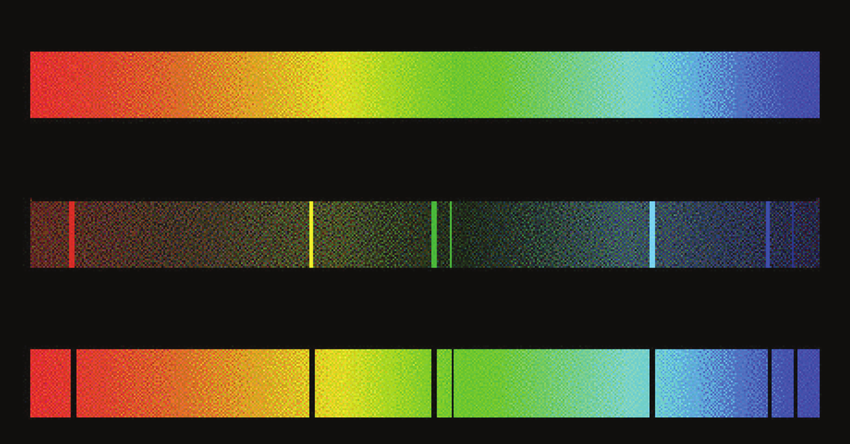
\includegraphics[width=10cm]{figuras/Continuous-spectrum-and-two-types-of-line-spectra.png}
\caption{Os três tipos de espectro: contínuo, de emissão e de absorção \citep{mcgrawhill}}
\label{fig:spectrum-types}
\end{figure}

% espectro estelar
Dentre esta grande variedade de objetos celestes, as estrelas são especialmente estudadas pelos seus espectros. Por serem objetos quentes, rodeados de gases mais frios (as chamadas atmosferas estelares), estrelas emitem um espectro de linhas de absorção sobreposto a um espectro contínuo. As linhas de absorção têm comprimentos de onda característicos dos elementos químicos que geraram o espectro. A figura~\ref{fig:vega-spectrum} ilustra o espectro da estrela Vega, cujo formato segue o de um espectro contínuo com a sobreposição de linhas de absorção de diversos elementos químicos.

\begin{figure}[htb]
\centering
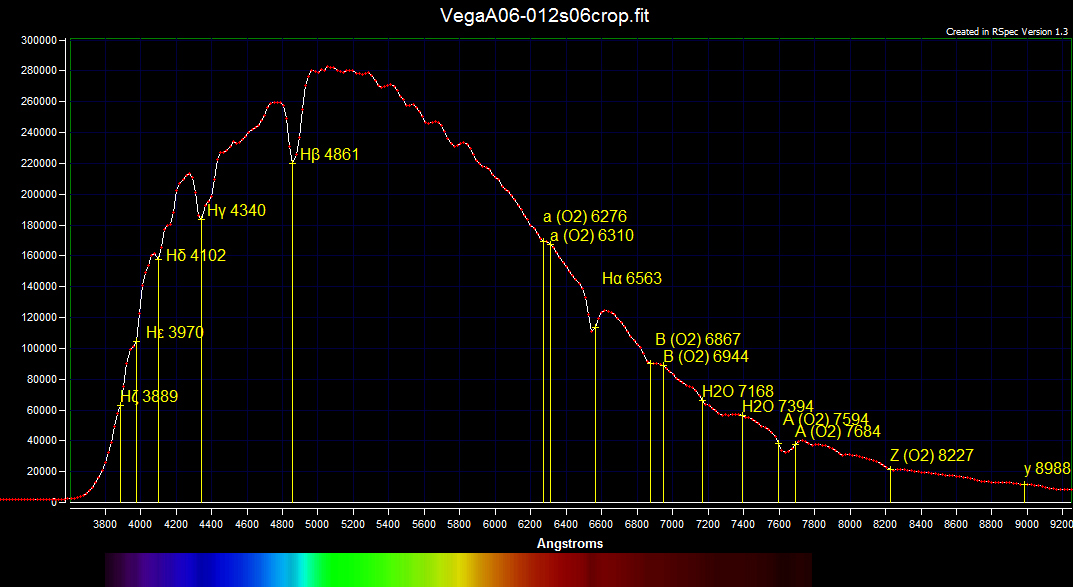
\includegraphics[width=12cm]{figuras/vega_spectrum.jpg}
\caption{O espectro da estrela Vega\citep{vega-spectrum}}
\label{fig:vega-spectrum}
\end{figure}

% história da classificação espectral e estudo dos espectros estelares
No final do século XIX, astrônomos perceberam que a análise cuidadosa do espectro de uma estrela fornece uma riqueza de detalhes sobre ela, incluindo sua temperatura efetiva, velocidade de rotação, velocidade de translação, densidade, composição química e metalicidade. Com a observação rotineira de espectros estelares em grandes números, estes pesquisadores notaram que era possível agrupar as estrelas com base em suas características espectrais, e assim surgiram diversos sistemas de classificação estelar. 

% sistema moderno de classificação espectral estelar
O sistema moderno de classificação de estrelas foi adotado em 1910 e foi criado por um time do observatório da Universidade de Harvard. Este sistema baseia-se nas intensidades relativas das linhas de absorção presentes no espectro. As variações nas linhas espectrais para diferentes estrelas são devidas principalmente à diferença de temperatura das camadas externas de gás na estrela, logo o sistema de classificação espectral é baseado na temperatura efetiva da estrela. 

% classes do sistema de classificação e relação com temperatura
As classes espectrais do sistema, em ordem decrescente de temperatura efetiva da estrela são O, B, A, F, G, K e M, como pode ser visto na tabela~\ref{tab:stellar-temperatures}. Cada uma dessas classes se divide em 10 subclasses (indicadas pelos números de 0 a 9), sendo 0 a mais quente dentro da classe e 9 a mais fria.
Na figura~\ref{fig:stellar-spectrum-types} é possível observar como diferentes linhas de absorção e bandas moleculares variam em intensidade conforme muda a temperatura efetiva, ou tipo espectral, da estrela.

\begin{table}[htb]
\centering
\begin{tabular}{|c|r|}
\hline
\textbf{Tipo Espectral} & \textbf{Temperatura efetiva (K)} \\ \hline
O                       & 30.000                               \\ \hline
B                       & 20.000                               \\ \hline
A                       & 10.000                               \\ \hline
F                       & 7000                                 \\ \hline
G                       & 6000                                 \\ \hline
K                       & 4000                                 \\ \hline
M                       & 3000                                 \\ \hline
\end{tabular}
\caption{A temperatura superficial estelar para cada tipo espectral \citep{iag-stellar-temps}}\label{tab:stellar-temperatures}
\end{table}

\begin{figure}[htb]
\centering
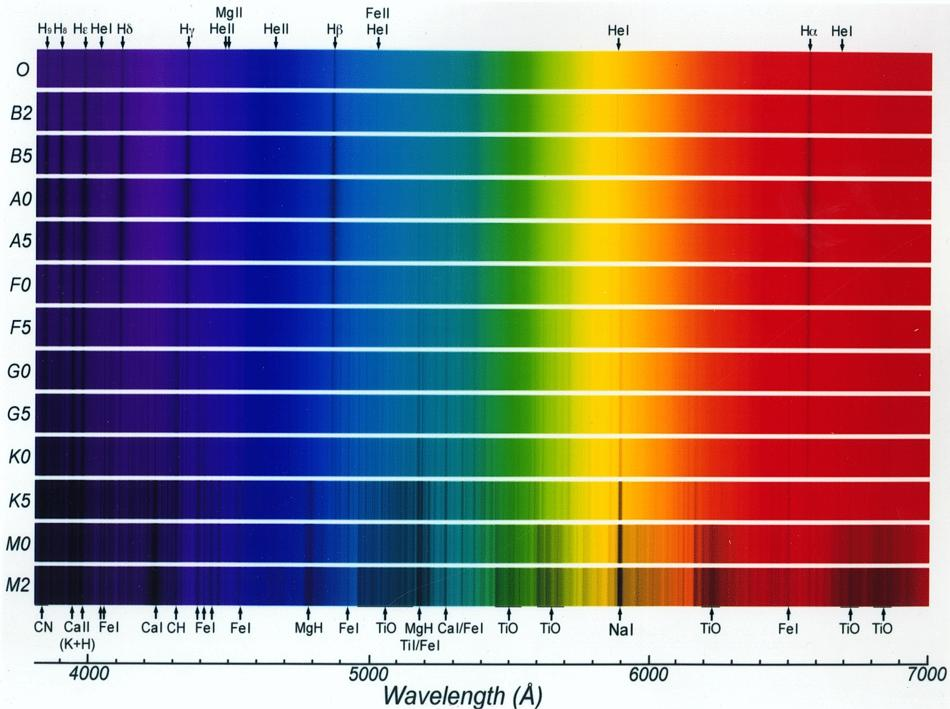
\includegraphics[width=10cm]{figuras/Spectra_Briley.jpg}
\caption{Tipos de espectro estelar \citep{astroprinceton}}
\label{fig:stellar-spectrum-types}
\end{figure}

% finalização da seção: aplicação em pesquisas atuais
% faltando referência
Os tipos espectrais das estrelas continuam sendo uma parte essencial para a pesquisa em astronomia, seja para auxiliar na descoberta de exoplanetas ou na interpretação da história da evolução das galáxias \citep{Charbonneau_2002}. 
% \pc{senti falta de uma referencia aqui. posso te ajudar, claro.}

% \pc{Pergunta para Isa e Marcelo: o quanto voces referenciam artigos em textos da Computacao? No texto abaixo, o meu impulso é adicionar uma referencia para cada conceito, como espectrografo, CCD etc... Posso ajudar nas referencias, claro, mas primeiro gostaria de saber se voces tb estao acostumados a adicionar referencia para quase cada conceito, ou se esse é um viés meu.}

% \mqz{Concordamos que qualquer afirmação que não seja clara para nosso leitor em potencial, ou que demande informações adicionais para ser justificada, deveria ser seguida por uma referência. A granularidade de ocorrência dessas referências poderia ser discutida: na passagem a seguir talvez uma referência por parágrafo fosse suficiente, considerando que os parágrafos estejam organizados em torno de uma ideia única central (que pode ser um conceito como sinal espectral ou redução de dados, ou ainda um dispositivo como CCD ou um banco de dados como o XShooter). Minha sensação inicial é que os parágrafos a seguir talvez não estejam tão claramente segmentados, ou seja, amarrados cada um a uma ideia central. Uma técnica que sempre me ajuda é preparar uma lista de ``bullet points'' sobre essas ideias; por exemplo, talvez na sequência a seguir essas ideias-aglutinadoras-de-parágrafos pudessem ser:
% \begin{itemize}
%     \item espectrógrafo e sinal espectral
%     \item redução de dados
%     \item descrição da coleção XShooter (isso me pareceria mais natural numa seção sobre datasets, mas talvez pudesse ser introduzida brevemente num parágrafo aqui como elemento auxiliar nas ilustrações dos demais conceitos teóricos).
% \end{itemize}
% Por sinal, tudo o que aparece nessa seção caberia muito naturalmente (mais naturalmente?) na seção~\ref{astronomic-spectroscopy} ``Espectrografia Astronômica''.}

\section{Redução de Dados}\label{data-reduction}

% importância instrumental na espectroscopia astronômica
Pesquisas na área de espectroscopia astronômica são dependentes de uma sólida estrutura instrumental. Isto significa que para coletar dados de objetos celestes é necessário ter acesso a instrumentos de observação, equipamentos de \textit{hardware} sofisticado que são capazes de transformar a radiação eletromagnética que alcança a superfície terrestre em dados cientificamente interpretáveis.

% ccd
Estes instrumentos de observação muitas vezes estão munidos de um CCD ou \textit{charge-coupled device}, um sensor eletrônico constituído por vários quadrados fotossensíveis, que registram o sinal em pixels de uma imagem. CCDs respondem linearmente ao sinal que os atinge e registram uma imagem da região do céu que está sendo observada. A chegada de cada fóton em um de seus pixels gera uma pequena carga elétrica armazenada para leitura posterior, e esta aumenta de forma proporcional à quantidade de fótons que atingem o aparelho \citep{davenhall20012}.

% pros e contras de ccd
Os benefícios de se usar um CCD para capturar imagens celestes é que eles automaticamente fornecem uma imagem digitalizada capaz de ser exibida e processada por um computador. Porém, estes dados brutos contêm uma série de assinaturas instrumentais que devem ser eliminadas antes que o dado possa ser usado para fins científicos \citep{davenhall20012}.  

% redução de dados
O processo de corrigir as imagens capturadas pelo CCD de suas assinaturas instrumentais é chamado de \textbf{\textit{redução de dados}} pela comunidade astronômica, e consiste de uma série de transformações aplicadas à imagem bruta. No final deste processo é obtida uma imagem científica utilizável e pronta para ser analisada.

% redução de dados no caso estelar
No caso dos espectros estelares, a redução de dados implica na extração de um espectro unidimensional a partir de uma imagem de CCD da estrela observada, também chamada de estrela de ciência. A figura~\ref{fig:calibration-steps}, ilustra as imagens de CCD antes e depois do processo de redução (painéis à esquerda e ao meio, respectivamente), e as representações dos espectros extraídos (painéis à direita).

% A figura~\ref{fig:x0319-obs-spectrum} ilustra o espectro de uma estrela da \textit{X-Shooter Spectral Library} \citep{Chen2014TheXS}, uma coleção de estrelas observada pelo espectrógrafo de resolução média \textit{X-Shooter}\footnote{\url{https://www.eso.org/sci/facilities/paranal/instruments/xshooter.html}}, parte do \textit{Very Large Telescope array}\footnote{\url{https://www.eso.org/public/brazil/teles-instr/paranal-observatory/vlt/?lang}} (VLT), localizado no Cerro Paranal, Chile.  

% \begin{figure}[htb]
% \centering
% 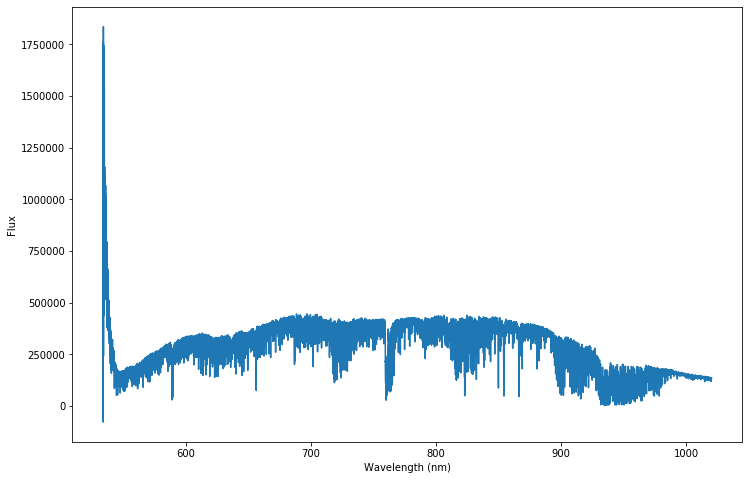
\includegraphics[width=15cm]{figuras/X0319_obs_spectrum.png}
% \caption{O espectro observado da estrela X0319}
% \label{fig:x0319-obs-spectrum}
% \end{figure}

\begin{figure}[htb]
\centering
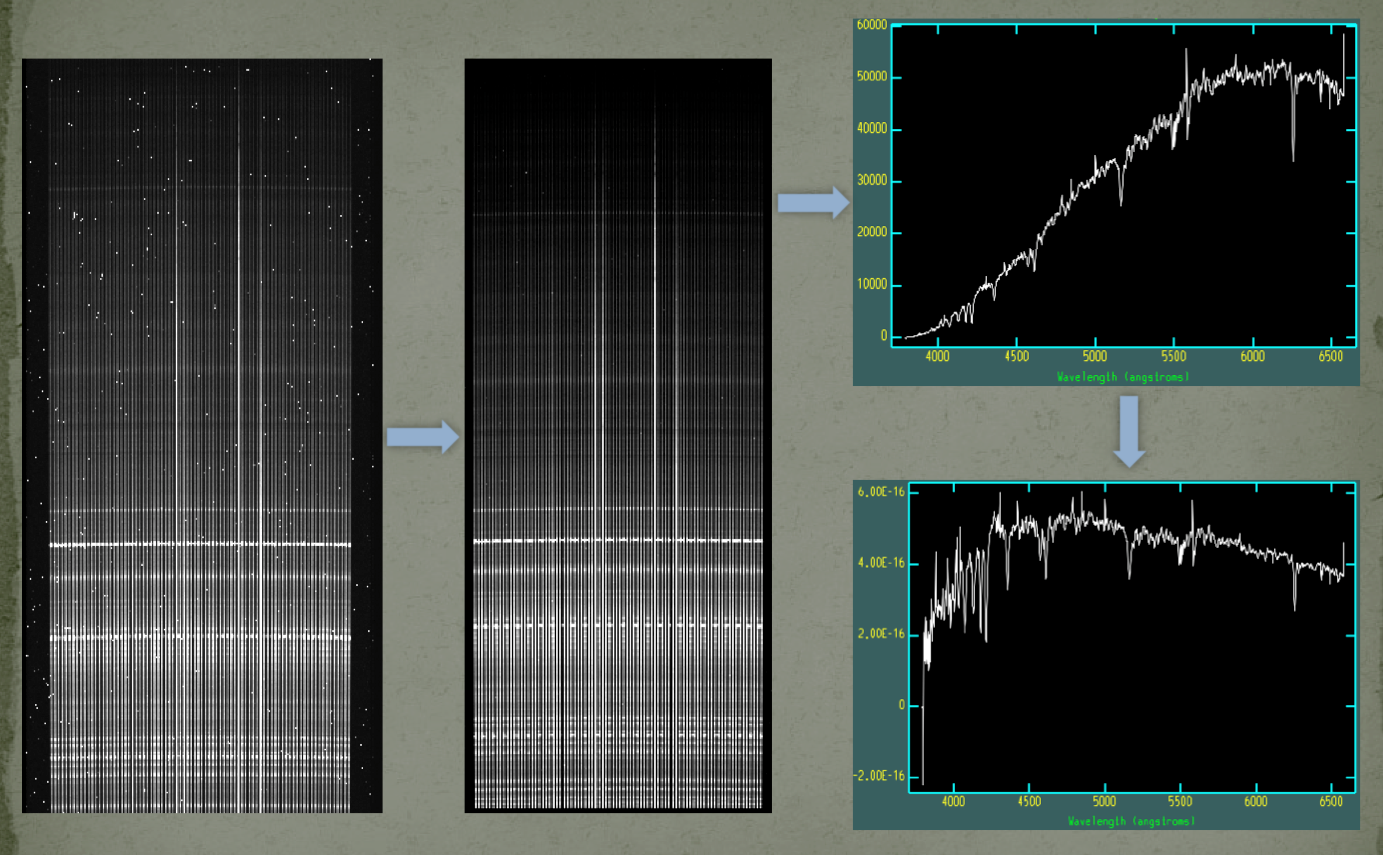
\includegraphics[width=15cm]{figuras/calibration_steps.jpg}
\caption{Redução de dados de uma imagem de CCD a um espectro unidimensional \citep{data-reduction-image}}
\label{fig:calibration-steps}
\end{figure}

% unidade do fluxo
O espectro resultante deste processo é unidimensional no domínio do comprimento de onda da estrela e tem sua intensidade representada por um fluxo, cuja unidade é erg/cm\(^{2}\)/s/Å, que representa a intensidade de energia por unidade de área, tempo e comprimento de onda \citep{astronomical-measurements}.

% tentativa da explicação da adimensionalidade do fluxo antes do final da redução de dados


% O fluxo é capturado em unidades de contagem de fótons, também chamadas de ADUs (\textit{Analog Digital Units}), que são adimensionais. O fluxo de um espectro estelar pode ser reescalonado para o intervalo $[0, 1]$, porém nem sempre isto é feito, como pode ser visto na imagem \ref{fig:x0319-obs-spectrum}. Também é possível observar que a figura \ref{fig:x0319-obs-spectrum} tem o formato esperado de um espectro estelar mencionado na seção \ref{astronomic-spectroscopy}: um espectro contínuo com a presença de várias linhas de absorção.


\section{Contaminação Telúrica} \label{telluric-contamination}

% voltar na menção da contaminação telúrica no começo do capítulo e juntar com a parte instrumental da seção anterior
Como mencionado na seção~\ref{astronomic-spectroscopy}, a maioria das observações astronômicas são feitas a partir do solo e, neste caso, nem toda luz irradiada por uma estrela consegue ser capturada por instrumentos de observação. 

% contaminação telúrica no observado
A principal consequência da interação da radiação eletromagnética estelar com a atmosfera terrestre é que novas linhas espectrais são formadas no espectro capturado instrumentalmente. As moléculas presentes na atmosfera terrestre formam linhas de absorção no espectro observado, denominadas de linhas telúricas.  

% como a atmosfera afeta certas regiões de comprimento de onda
No espectro estelar, regiões diferentes de comprimentos de onda possuem diferentes sensibilidades à atmosfera. Isso implica que em certas regiões do espectro de ciência existe uma maior presença das linhas telúricas do que em outras. Na figura~\ref{fig:molectfit-telluric-reference}, é possível ver estas linhas telúricas e suas respectivas moléculas responsáveis em uma grande extensão de comprimentos de onda.

%% INCLUIR FIGURA DA LITERATURA AQUI %%
\begin{figure}[!htb]
\centering
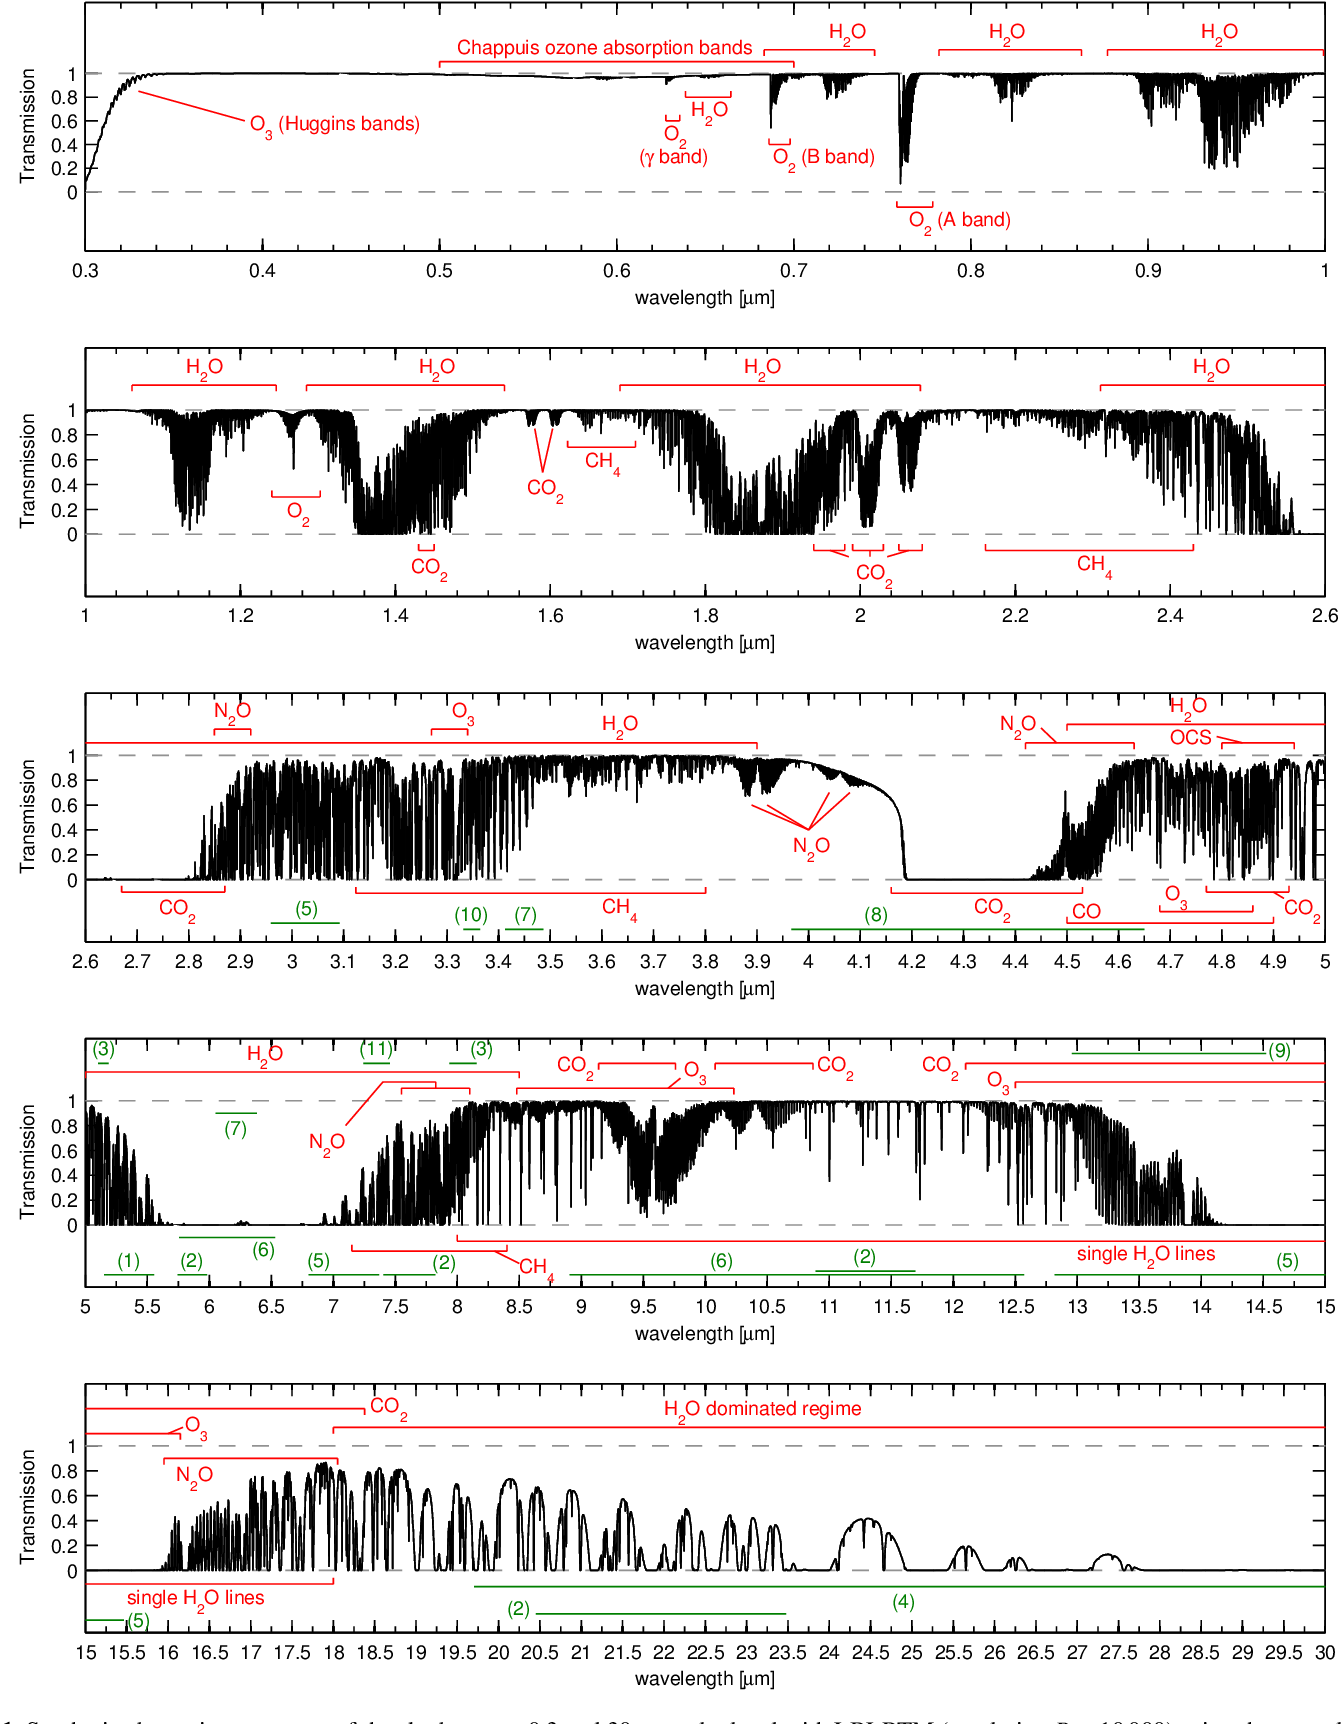
\includegraphics[width=15cm, trim=0 10 0 0, clip]{figuras/telluric_reference_molecfit.png}
\caption{Espectro de absorção sintético criado pelo \texttt{Molecfit} que ilustra como diferentes moléculas interagem com diferentes regiões de comprimento de onda \citep{smette2015molecfit}}
\label{fig:molectfit-telluric-reference}
\end{figure}

% Como as estrelas do \textit{X-Shooter Spectral Library}, a maioria das observações astronômicas são feitas em telescópios terrestres, ou seja, a partir do solo. Nesse caso, nem toda luz irradiada por um objeto celeste pode ser capturada pelo espectrógrafo. Isto acontece porque, ao atravessar a atmosfera terrestre, o sinal astronômico interage com moléculas como vapor de água e oxigênio, o que resulta na formação de novas linhas de absorção no espectro observado, chamadas de linhas telúricas. 

% \pc{acho que cabe mencionar que regioes diferentes de comprimento de onda sao mais ou menos sensiveis aa atmosfera, e mostrar um grafico ilustrando um espectro telurico. pode ser da literatura, assim mostramos um observado (ao contrario dos que voce tem sao modelos). }

% efeitos da contaminação telúrica no espectro
As linhas telúricas  contribuem para a criação de uma observação distorcida ou contaminada. A menos que seja corrigida, esta contaminação pode produzir erros de interpretação e ruídos que reduzem a precisão dos dados observados, e consequentemente, dificultam o avanço de diversas pesquisas astronômicas.

% procedimentos atuais para correção telúrica
Existem alguns procedimentos típicos usados hoje em dia para remover as linhas telúricas de um espectro de ciência. Um método popular consiste em aplicar uma divisão simples entre o espectro da observação e uma referência telúrica, que consiste em uma função representando a transmissão radiativa da atmosfera terrestre para cada comprimento de onda, desde que satisfeita a condição de que o referencial telúrico tenha as mesmas assinaturas instrumentais do espectro de ciência. Esta referência telúrica pode ser obtida de duas maneiras: através da observação de uma estrela padrão, ou pela simulação de um espectro atmosférico teórico, conforme detalhado a seguir.

% estrelas padrão
As estrelas padrão são estrelas quentes em rotação rápida de tipo espectral B ou A. Elas são escolhidas pois seus espectros não possuem características marcantes além de fortes linhas de hidrogênio. Para que o espectro de uma estrela padrão seja usado como uma referência telúrica, é necessário observá-la em condições muito próximas (tempo, posição no céu e condições atmosféricas) daquelas referentes ao espectro de ciência. Contudo, existem várias limitações fundamentais no nível de correção que pode ser obtido com o método da estrela padrão. Primeiramente, outras características estelares além das linhas de hidrogênio ainda podem estar presentes no espectro da estrela padrão, evidenciando que ela não é um modelo preciso da transmissão radiativa da atmosfera. Além disso, o tempo e a direção de observação das duas estrelas nunca será exatamente o mesmo, o que significa que a assinatura atmosférica de ambos os espectros também será necessariamente diferente.

% espectros de transmissão atmosférica sintéticos
Devido às limitações no uso das estrelas padrão, foi criado um método mais sofisticado e automatizado para produzir uma referência telúrica: softwares de simulação do espectro atmosférico. Estes softwares utilizam modelos de transmissão radiativa da atmosfera para criar um espectro telúrico sintético, cujas condições de simulação são muito próximas às condições de observação da estrela de ciência. O modelo de transmissão atmosférica mais utilizado hoje em dia é o \textit{Line-By-Line Radiative Transfer Model (LBLRTM)} \citep{2005JQSRT..91..233C}, que fornece cálculos de radiância espectral com precisão e eficiência. Este modelo utiliza o HITRAN \citep{rothman2009hitran}, um acrônimo para \textit{High-resolution Transmission molecular absorption database}, uma base de dados de linhas e parâmetros espectroscópicos. 

% exemplo do molecfit
Um exemplo de software de simulação do espectro atmosférico é o \texttt{Molecfit} \citep{smette2015molecfit}, uma ferramenta para a modelagem de linhas telúricas desenvolvido por astrônomos do \textit{European Southern Observatory}\footnote{\url{https://www.eso.org/public/}}. De acordo com seus criadores, o \texttt{Molecfit} recupera o perfil atmosférico mais compatível com o instante da observação da estrela de ciência. Isto envolve a utilização de um modelo de transmissão radiativa da atmosfera com uma base de dados de condições atmosféricas para recuperar atributos como a variação na temperatura, pressão e umidade em função da altitude da observação.

% o que o referencial telúrico representa em termos da absorção da radiação pela atmosfera
Independentemente de como é gerado o referencial telúrico, considera-se que ele representa coeficientes de transmissão da radiação através da atmosfera, no sentido que, para cada comprimento de onda, a quantidade de radiação propagada desde a estrela que consegue atravessar a atmosfera e chegar ao instrumento é dada em percentual, representado pelo coeficiente de transmissão\footnote{Isso está de acordo com o princípio da superposição e equivale à hipótese de linearidade do processo de transmissão radiativa no vácuo, sob a qual a transmissão pode ser modelada independentemente para cada frequência ou comprimento de onda.}. %\mqzinline{Paula, você poderia ler e verificar se esse trecho (+footnote) tem algum erro grosseiro?}

% operacionalização do problema da contaminação telúrica
Em termos matemáticos, consideramos os espectros de ciência, telúrico e estelar sem contaminação como vetores $o$ (observado), $a$ (atmosfera) e $s$ (estrela),

\begin{equation*}
    o = (o_1, o_2, \cdots, o_{n}) \qquad a = (a_1, a_2, \cdots, a_{n}) \qquad s = (s_1, s_2, \cdots, s_{n}), 
\end{equation*}

\noindent representando valores discretos do fluxo estelar ou atmosférico em $n$ comprimentos de onda específicos (geralmente equi-espaçados). A contaminação telúrica do espectro de ciência se refere então à equação

\begin{equation*}
    o = a \circ s \qquad \left(\mbox{ou equivalentemente:} \qquad o_i = a_i\cdot s_i,\ \forall i\right),
\end{equation*}

\noindent onde o símbolo $\circ$ representa o produto de Hadamard entre o espectro estelar original e o referencial telúrico, e a equação pressupõe que as três sequências estejam perfeitamente alinhadas, ou seja, que cada índice $i$ represente o mesmo comprimento de onda nos três espectros. Esse é um possível ponto de partida para o tratamento dos espectros estelares com técnicas computacionais associadas ao processamento de sinais digitais, abordadas a seguir.
%Esta representação tem como objetivo relaxar as restrições físicas do problema, de forma que seja possível aplicar algoritmos nos sinais que dependem da suposição de linearidade da contaminação telúrica.


\section{Similaridade e alinhamento de sinais}\label{similarity-and-signal-alignment}

% processamento de sinais e similaridade
O processamento de sinais digitais tem como foco extrair informações significativas dos sinais, bem como modificá-los a fim de atingir determinados objetivos. Uma das operações importantes na análise de sinais digitais é a mensuração da similaridade entre dois sinais. Medidas de similaridade possuem diversas aplicações em áreas como reconhecimento de fala, para saber se um sinal de voz corresponde a um determinado texto, ou em economia, para comparar investimentos em períodos diferentes, entre outras aplicações.

% possiveis problemas na operacionalização do problema como descrito acima (mencionar os três problemas)
Como foi mencionado na seção~\ref{telluric-contamination}, é possível assumir que o problema da contaminação telúrica pode ser operacionalizado como uma multiplicação simples partindo do pressuposto de que os sinais se encontram em uma situação ideal. Estabelece-se como uma situação ideal os sinais que: (i) possuem mesma intensidade, ou seja, que foram observados com as mesmas condições atmosféricas (pressão, temperatura, umidade, turbulência etc); (ii) possuem mesma assinatura instrumental; (iii) são amostrados nos mesmos comprimentos de onda, ou seja, estão perfeitamente alinhados pixel a pixel. 

% contexto do desalinhamento nos dados observados XSL
Nesse trabalho, optamos por estudar a questão do alinhamento do sinal, motivados por uma dificuldade real que foi encontrada por um grupo de pesquisadores envolvidos na \textit{X-Shooter Spectral Library} \citep[][XSL]{Chen2014TheXS}. A XSL é uma coleção de estrelas observada pelo espectrógrafo de resolução média \textit{X-Shooter}\footnote{\url{https://www.eso.org/sci/facilities/paranal/instruments/xshooter.html}}, do ESO. Essa biblioteca de estrelas tem diversas aplicações em Astronomia, desde o estudo de abundâncias químicas de estrelas da nossa Galáxia até a modelagem evolutiva de outras galáxias. Pesquisadores que usaram estes dados para suas pesquisas relataram desalinhamentos nos comprimentos de onda dos espectros \citep{unpublished-xshooter-data-release, wavelength-shifts}.

\begin{figure}[htb]
\centering
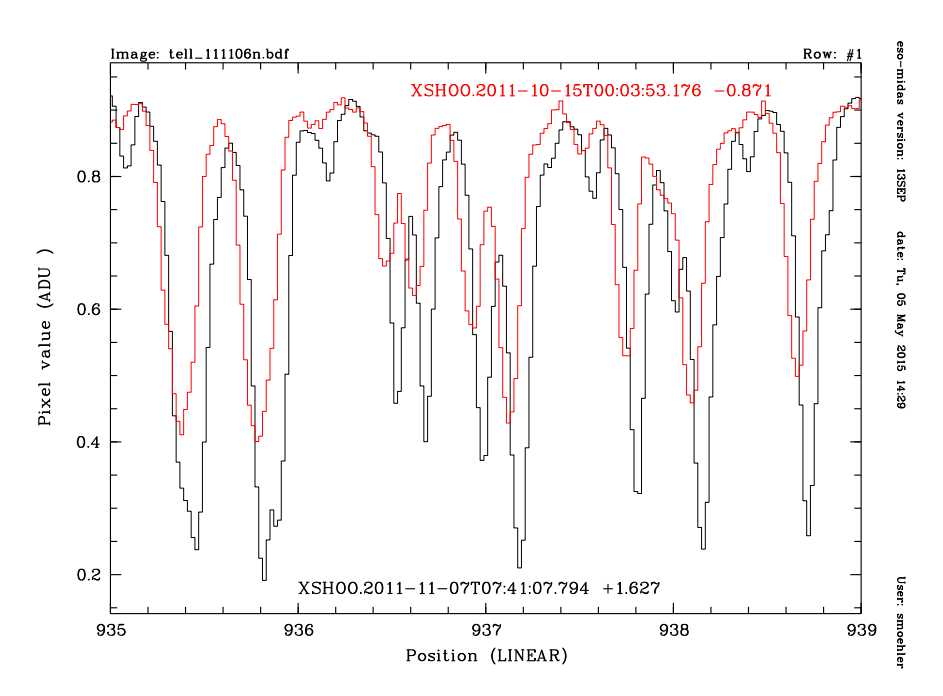
\includegraphics[width=12cm]{figuras/xsl-wavelength-shifts.png}
\caption{Desalinhamentos observados nos espectros telúricos do XSL \citep{wavelength-shifts}}
\label{fig:matlab-dtw}
\end{figure}

% similaridade no contexto dos espectros estelares
Diante disso, é possível entender porque o estudo da similaridade entre sinais pode ser útil em espectros estelares: para alinhar regiões de contaminação atmosférica de moléculas específicas em um espectro de ciência com as regiões correspondentes no espectro telúrico. Em teoria, isto melhoraria o resultado da divisão entre o espectro de ciência observado e o telúrico, e consequentemente, a qualidade do espectro estelar sem contaminação.

% distancia euclideana e metricas de similaridade
Uma medida tradicional de diferença entre informações numéricas que poderia ser usada como medida de similaridade entre dois sinais digitais é a distância euclideana entre os vetores correspondentes. Porém em sinais com flutuações rápidas é fácil perceber que mesmo um pequeno desalinhamento poderia provocar um grande aumento na distância entre os sinais.

% introdução a DTW
Um algoritmo robusto utilizado para determinar a similaridade entre dois sinais digitais é o \textit{Dynamic Time Warping (DTW)}. Este algoritmo acha uma correspondência ótima entre os índices de dois vetores, de tal maneira a minimizar as distâncias entre os índices correspondentes. Essa correspondência equivale a um alinhamento entre as sequências que torna os sinais realinhados mais similares~\citep{shou2005fast}. 

% explicacao da dtw pela imagem 
A figura~\ref{fig:matlab-dtw} ilustra o alinhamento ótimo encontrado pelo DTW entre um sinal cuja frequência aumenta com o tempo e uma sinusoide. O alinhamento encontrado corresponde à distância euclideana mínima entre as duas sequências, de forma que regiões com formatos similares estejam o mais próximas possíveis no alinhamento.

\begin{figure}[htb]
\centering
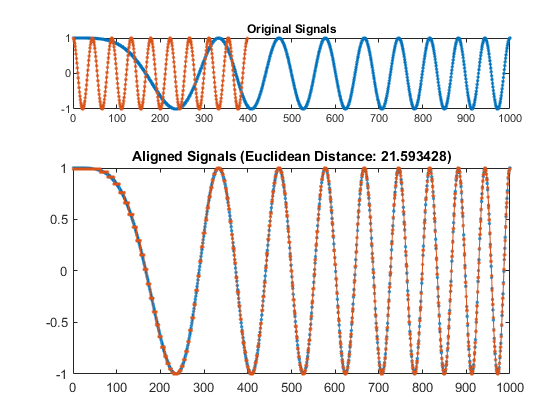
\includegraphics[width=12cm]{figuras/DynamicTimeWarpingOfRealChirpAndSinusoidExample_01.png}
\caption{Sinais originais e alinhados com a DTW com a distância euclideana final \citep{matlab-dtw}}
\label{fig:matlab-dtw}
\end{figure}

% formulacao matematica do problema
\newcommand{\dist}{\mbox{dist}}

A formulação do problema \citep{salvador2007toward} do DTW é a seguinte: dadas duas sequências $X$ e $Y$, de comprimentos respectivos $n$ e $m$,
\begin{align*}
    X = (x_1, x_2, \cdots, x_n) \\
    Y = (y_1, y_2, \cdots, y_m),
\end{align*}

construa um caminho $W$ de comprimento $k$

\begin{equation*}
    W = (w_1, w_2, \cdots, w_k), \qquad max(n, m) \leq k < n + m,
\end{equation*}

\noindent que satisfaça as seguintes condições:

\begin{itemize}
\item o $k$-ésimo elemento do caminho $W$ é $w_k = (i_k, j_k)$, onde $i_k$, $j_k$ são índices das sequências $X$ e $Y$, respectivamente;
\item o caminho $W$ deve começar em $w_1 = (1, 1)$ e deve terminar em $w_k = (n, m)$, de forma a assegurar que todos os índices das duas sequências serão usados;
\item o caminho $W$ força $i_k$ e $j_k$ a serem monótonos não-decrescentes como funções de $k$; em termos matemáticos isso equivale a
\begin{equation*}
    i_k \leq i_{k+1} \leq i_k + 1 \qquad \mbox{e} \qquad j_k\leq j_{k+1} \leq j_k + 1;
\end{equation*}
\item o caminho $W$ minimiza a função 
\begin{equation*}
    \dist(W) = \sum_{n=1}^{k} \dist(x_{i_n}, y_{j_n})
\end{equation*}
onde $\dist(x_{i_n}, y_{j_n})$ é uma medida de distância, tipicamente a euclideana, entre um par de elementos das sequências $X$ e $Y$.
\end{itemize}

As três primeiras condições definem uma enorme quantidade de caminhos/alinhamentos possíveis, ao passo que a quarta condição estabelece um critério de comparação entre dois alinhamentos distintos.

% implementacao do dtw
A implementação do algoritmo utiliza o paradigma da programação dinâmica, onde cada instância do problema é resolvida combinando soluções de subproblemas da instância original. O diferencial desta abordagem é que os resultados dos subproblemas são armazenados em uma tabela ou matriz. No caso da DTW é criada uma matriz de distâncias acumuladas $D$, de dimensão $n \times m$, onde $D(i, j)$ armazena o valor da distância total do caminho mínimo que pode ser construído entre as subsequências $X' = \{x_1, \cdots, x_i\}$ e $Y' = \{y_1, \cdots, y_j\}$. Logo, o valor armazenado em $D(n, m)$ representa a distância do caminho mínimo que compreende as duas sequências inteiras. O preenchimento da matriz $D$ é feito da seguinte forma:

\begin{equation*}
    D(i, j) = \left\{\begin{array}{ll}
    \displaystyle\sum_{k=1}^j\dist(x_1,y_k)&\mbox{se\ }i=1\\
    \displaystyle\sum_{k=1}^i\dist(x_k,y_1)&\mbox{se\ }j=1\\
    \dist(x_i, y_j) + \min\{D(i - 1, j), D(i, j - 1), D(i - 1, j - 1)\}&\mbox{caso contrário}
    \end{array}\right.
\end{equation*}

% pros da abordagem de programacao dinamica e descricao do algoritmo
Esta abordagem funciona pois, ao se calcular $D(i,j)$, todos os caminhos ótimos de subsequências menores do que as sequências de tamanhos $i$ e $j$ já foram considerados, logo, a distância armazenada em $D(i, j)$ corresponde à distância mínima entre todos os caminhos possíveis para subsequências com apenas um índice de diferença em relação a $i$ ou $j$ (ou ambos), mais a distância entre o par $x_i$ e $y_j$. A inicialização da linha $i=1$ e da coluna $j=1$ explora o fato de que para alinhar uma subsequência qualquer de X (ou Y) com apenas um elemento do outro vetor, o único caminho possível é aquele que alinha todos os elementos da subsequência ao único elemento possível.

% backtrack para encontrar caminho na matriz
Depois que a matriz $D$ está completa, é necessário reconstruir um caminho ótimo entre $D(1, 1)$ e $D(n, m)$, pois a matriz só traz esse caminho de forma implícita, através dos mínimos que foram considerados no cálculo de $D(i,j)$. Essa reconstrução é feita na ordem inversa: a partir do final do caminho $D(n, m)$, consideram-se os elementos à esquerda $D(n,m-1)$, abaixo $D(n-1,m)$ e na diagonal inferior esquerda $D(n-1,m-1)$; dentre estes, o elemento com o menor valor é adicionado ao caminho ótimo como antecessor de $D(n,m)$. Este procedimento é repetido até que o caminho chegue na posição $D(1, 1)$.

\begin{figure}[htb]
\centering
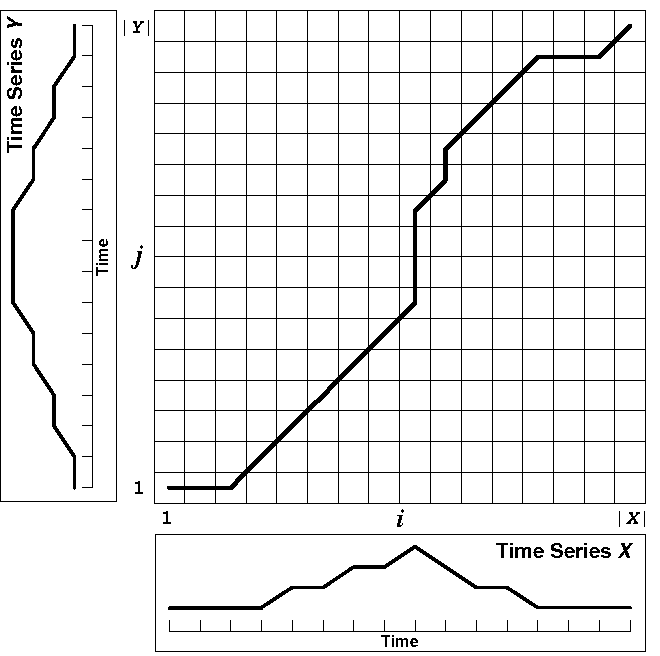
\includegraphics[width=9cm]{figuras/dtw_warp_path.png}
\caption{Uma matriz de similaridade com o caminho ótimo da DTW entre as séries X e Y\citep{salvador2007toward}}
\label{fig:dtw-matrix-and-path}
\end{figure}

O pseudo-código dos procedimentos de preenchimento da matriz \citep{hierarchical-time-clustering} e de \textit{backtracking} que compõem a DTW são dados pelos algoritmos \ref{dtw-matrix} e \ref{dtw-path}.

\begin{algorithm}
\caption{DTW matrix filling}\label{dtw-matrix}
\begin{algorithmic}[1]
\Procedure{DTW}{$x,y$}
    \Comment{Seja $M$ uma matriz bidimensional $n \times m$}
    \State $M[0, 0]\gets 0$
    \For{$i \gets 1$ to $m$}
        \State $M[0, i] \gets \infty$
    \EndFor
    \For{$i \gets 1$ to $n$}
        \State $M[i, 0] \gets \infty$
    \EndFor
    \For{$i \gets 1$ to $n$}
        \For{$j \gets 1$ to $m$}
            \State $d = \dist(x[i], y[j])$
            \State $M[i, j] = d + min(M[i-1, j], M[i, j-1], M[i-1, j-1])$
        \EndFor
    \EndFor
\State \textbf{return} $M[n, m]$\Comment{Distância do caminho ótimo}
\EndProcedure
\end{algorithmic}
\end{algorithm}

\begin{algorithm}
\caption{DTW path backtracking}\label{dtw-path}
\begin{algorithmic}[1]
\Procedure{DTW\_path}{$M$}
    \Comment{Seja $P$ uma lista de tuplas}
    \State $i\gets n$
    \State $j\gets m$
    \While{$i \neq 0$ and $j \neq 0$}
        \State P.add(i, j)
        \If{$M[i-1, j-1] \leq M[i-1, j]$ and $M[i-1, j-1] \leq M[i, j-1]$}
            \State $i \gets i - 1$
            \State $j \gets j - 1$
        \ElsIf{$M[i-1, j] \leq M[i-1, j-1]$ and $M[i-1, j] \leq M[i, j-1]$}
            \State $i \gets i - 1$
        \Else
            \State $j \gets j - 1$
        \EndIf
    \EndWhile
\State \textbf{return} $P$\Comment{Índices do caminho ótimo}
\EndProcedure
\end{algorithmic}
\end{algorithm}

% analise da complexidade dtw
É possível analisar a complexidade de tempo e espaço da DTW com o algoritmo de preenchimento da matriz de similaridade. Cada elemento da matriz $n \times m$ é escrito exatamente uma vez em tempo constante, e a matriz inteira é armazenada na memória. Logo, ambas as complexidades são $\mathcal{O}(nm)$, que no caso de $n = m$, equivale a uma complexidade assintótica $\mathcal{O}(n^2)$. A complexidade de espaço é especialmente proibitiva, visto que sequências obtidas de espectros estelares com apenas 177 mil elementos geram uma matriz de similaridades que exige \textit{terabytes} de memória para ser armazenada.

% contras da complexidade quadratica
A complexidade quadrática tanto em tempo quanto em espaço da DTW cria a demanda por métodos que consigam acelerar este procedimento. No artigo de \citet{salvador2007toward}, é proposta uma abordagem multinível inspirada no problema da partição de grafos. Essa técnica tende a funcionar bem para problemas muito grandes e de difícil solução exata. Neste caso, soluções de problemas menores ou parciais podem ser refinadas e combinadas para que se encontre uma boa aproximação da solução do problema original.

% fast dtw e descricao do algoritmo
O algoritmo proposto, chamado de \textit{FastDTW}, depende de algumas operações-chave: a redução das séries temporais, a projeção do caminho da DTW para maiores resoluções e o refinamento do caminho encontrado. A redução das séries temporais é feita tirando a média de pontos adjacentes e o resultado são vetores com a metade do seu comprimento original. Repete-se esta operação várias vezes para se criar todas as resoluções das séries temporais que serão usadas, de maneira similar à transformada Wavelet. O algoritmo quadrático padrão da DTW é utilizado para as séries temporais com menor resolução e o caminho ótimo encontrado é então projetado para a próxima maior resolução que foi computada. Na projeção aplica-se uma versão restrita da DTW apenas na vizinhança próxima do caminho resultante da projeção, o que não garante que o caminho ótimo será encontrado. Para aumentar as chances de encontrar a solução ótima existe um parâmetro de raio $r$, que representa o número de células adjacentes ao caminho projetado que farão parte da DTW restrita. Este procedimento é repetido para todas as resoluções até se obter um caminho na resolução original.

% estrategia recursiva e complexidade assintotica
O algoritmo usa uma estratégia recursiva, na qual o caso base é o uso da DTW quadrática padrão em uma resolução bastante baixa dos sinais. Uma análise da complexidade de tempo e espaço do pior caso em que ambas as séries temporais possuem $n$ elementos, resulta em $n(8r + 14)$ para tempo e $n(4r + 7)$ para espaço, ou seja, se o parâmetro $r$ é um valor constante pequeno ($\ll n$), podemos afirmar que as complexidades assintóticas são $\mathcal{O}(n)$.

% algoritmo de realinhamento feito por nós 
Como pode ser visto nos algoritmos \ref{dtw-matrix} e \ref{dtw-path}, as saídas do DTW são a distância e o caminho ótimo entre duas sequências. Neste trabalho foi produzido um algoritmo que tem como objetivo produzir sequências alinhadas. Para isso é utilizado o caminho resultante da DTW e é feita uma aproximação do realinhamento de uma das sequências em relação à outra. O algoritmo implementado usa os índices repetidos no caminho da DTW e tira a média entre os elementos correspondentes para criar um valor representativo da correspondência de uma região maior de uma sequência com uma região menor de outra.

% descricao matematica do realinhamento
Em termos matemáticos temos as sequências $a$ e $o$, definidas na seção \ref{telluric-contamination}, e queremos construir um $\overline{a}$ que representa a sequência $a$ realinhada em relação à sequência $o$, a partir de um caminho $P$ obtido pelo DTW. Os caminhos construídos pelo algoritmo DTW podem associar cada índice de uma sequência a vários índices adjacentes da outra sequência. Para contornar essa questão na construção de $\overline{a}$, foi definido o seguinte procedimento: para cada índice $l=0,\ldots,n$ da sequência $o$, define-se

\begin{equation*}
    \overline{a}_l = \mbox{média} \{a_k\}_{k \in L}
\end{equation*}

\noindent onde

\begin{equation*}
  L = \{m | (m, l) \in P\}
\end{equation*}

\noindent e $P$ representa o caminho resultante da DTW entre $a$ e $o$. O pseudo-código correspondente a essa definição pode ser visto no algoritmo \ref{dtw-realignment}

\begin{algorithm}[H]
\caption{Sequence alignment}\label{dtw-realignment}
\begin{algorithmic}[1]
\Procedure{align\_sequence\_dtw\_path}{$P$, $s$}
    \Comment{Seja $P$ uma lista de tuplas e $s$ o vetor a ser realinhado}
    \State $d \gets \emptyset$ \Comment{Seja $d$ uma associação chave-valor vazia}
    \State $aligned \gets \emptyset$
    \For{$(i, j)$ in $P$}
        \State insere $i$ na lista $d[j]$
    \EndFor
    \For{$(j, lista)$}
        \State $m \gets$ média dos valores de $s$ associados aos índices na lista $d[j]$
        \State $aligned[j] \gets m$
    \EndFor
\State \textbf{return} $aligned$\Comment{Sequência realinhada}
\EndProcedure
\end{algorithmic}
\end{algorithm}

Os procedimentos descritos acima serão explorados nos experimentos apresentados no próximo capítulo.